
\textbf{Data and Ethics}. We use CHUR-XP2 (OpenNeuro ds002338) \citep{lioi2019simultaneous}: simultaneous EEG--fMRI from 17 healthy participants, motor-imagery run after neurofeedback training (\texttt{MIpost}), a block design with the same timing for every participant. EEG: 63 scalp channels and one ECG lead, corrected for gradient and pulse artefacts; fMRI: TR 1\,s, a 16-slice slab, resized to $64\times64\times30$. We replicate the main analyses on the motor-localizer run of CHUR-XP1 (ds002336; 9 subjects, TR 2\,s). Both public, de-identified datasets were acquired with ethical approval and informed consent \citep{lioi2019simultaneous}; this secondary analysis required no additional approval.

\subsection{EEG-conditional protocol}\label{sec:problem}

Each subject $s$ has pairs $(x_{s,t}, y_{s,t})$, where $y_{s,t}$ is the fMRI volume at time $t$ and $x_{s,t}$ the short-time Fourier magnitude of the EEG over the 10\,s before it. A synthesizer is a predictive distribution $p_\theta(y\mid x)$, trained and tested on disjoint subjects. We score it with the negative log-likelihood (NLL), the continuous ranked probability score (CRPS) \citep{gneiting2007strictly} and the root mean square error (RMSE) over a brain mask fixed from the training subjects, together with interval coverage, the Spearman correlation between predictive standard deviation (SD) and error, and sparsification (Supplementary Section~S2). Subjects, not volumes, are the unit of every test. A synthesizer is \emph{informative about the EEG} only if it passes two comparisons.

The \emph{EEG-free references} define the null hypothesis that a model uses no EEG information; we reject it only if the model scores better than all of these predictive distributions, which never see EEG:
\begin{itemize}
	\item \textbf{population template}: a voxelwise Gaussian distribution with the mean and standard deviation of all training volumes;
	\item \textbf{stimulus-locked template}: the same moments at each volume index, which predicts the task response without EEG;
	\item \textbf{own-subject oracle}: with the test subject's own voxel moments, an upper bound that uses test data.
\end{itemize}

We also compare the EEG based models with \emph{EEG nulls}. These models are evaluated with their input replaced by:
\begin{itemize}
	\item a \textbf{shift null}, the subject's EEG circularly shifted by at least 30 volumes, complementary to the IAAFT surrogates of \citet{mehta2025eegbold}, which randomize the phases of the BOLD instead;
	\item a \textbf{swap null}, another test subject's EEG at the same volume index.
\end{itemize}
We compare the median voxel temporal correlation $r$ between predicted and observed time courses. Beating the shift null but not the swap null means the model learned something locked to the shared task timing, not to the subject's EEG.

All comparisons use one-sided paired Wilcoxon tests over subjects at $\alpha=0.05$. Every claim of absence is backed by a Hodges--Lehmann estimate with a bootstrap 95\% confidence interval (CI) and a non-superiority test against a smallest effect of interest fixed in advance: $0.05$ in $r$, and 5\% of the template--oracle gap in NLL, CRPS and RMSE. Conformal intervals are calibrated on two held-out subjects per fold, and cross-conformally on all other subjects.

\subsection{Synthesizers}\label{sec:methods}
All networks share the encoder of \citet{calhas2022eeg}, whose architecture was found by neural architecture search \citep{calhas2021automatic} and is kept fixed. Only the decoder differs between methods.

\paragraph{Spectral relaxation.} We propose a low resolution prediction produced by the discrete cosine transform (DCT) \citep{ahmed1974discrete}, which pads the coefficients with zeros to full size and inverts the transform (Fig.~\ref{fig:upsampling_dct}). With a relaxation factor $\kappa=2$ it predicts $32\times32\times15$ instead of $64\times64\times30$ values, on the premise that EEG cannot inform the full resolution of the fMRI \citep{burle2015spatial}. Every output then lies in the span of the retained DCT basis, so the orthogonal projection onto that span gives an exact bound on what any relaxed decoder can express.

\begin{figure}[ht]
	\centering
	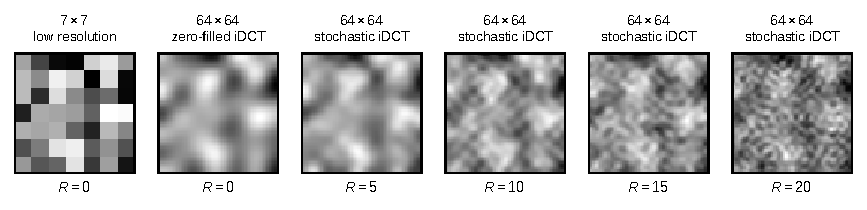
\includegraphics[width=\textwidth]{figures/dct_upsampling.pdf}
	\caption{Upsampling through the DCT, from $7\times 7$ to $64\times 64$. Left to right: the low-resolution image, its zero-filled upsampling, and upsamplings with an increasing number of Gaussian random coefficients above the cutoff.}
	\label{fig:upsampling_dct}
\end{figure}

\paragraph{Stochastic spectral decoder.} Our UQ method makes the relaxed decoder stochastic in the DCT domain (Fig.~\ref{fig:spectralUpsampling}). The retained coefficients are multiplied by Gaussian gains, and every coefficient above the cutoff is a sum of $H=20$ sinusoids of von Mises variables, weighted by an attention over the low coefficients. Its samples span the full resolution. Its noise parameters are trained by maximum likelihood without a prior, so we score it as a predictive distribution (Supplementary Section~S3).

\begin{figure*}[!htbp]
    \centering
    \begin{tikzpicture}[scale=3]
        \node (xaxis) at (3.2,0) {$r$};
        \node (yaxis) at (-0.1,1) {$p$};
        %axes
        \draw ($(xaxis)+(-3.2,0)$) -- ($(xaxis)+(-0.65,0)$);
        \node (dots) at ($(xaxis)+(-0.5,0)$)  {$\dots$};
        \draw[->]  ($(xaxis)+(-0.35,0)$) -- ($(xaxis)+(-0.1,0)$);
        \draw[->] ($(yaxis)+(0.1,-1.1)$) -- ($(yaxis)+(0.1,0)$);
        
        \node (origin) at (0,0) {};
        
        \draw[bottom color=blue,top color=blue!10, draw=blue] ($(origin)+(0.1,0)$) .. controls +(0,0) and +(0,0) .. ($(origin)+(0.1,0.5)$) .. controls +(0.5,0.5) and +(-0.2,0.5) .. ($(origin)+(1.5,0.5)$) .. controls +(0,0) and +(0,0) .. ($(origin)+(1.5,0)$);
        
        
        \draw[bottom color=yellow,top color=yellow!10, draw=orange] ($(origin)+(1.5,0)$) .. controls +(0,0) and +(0,0) .. ($(origin)+(1.5,0.5)$) .. controls +(0.4,-0.7) and +(-0.2,0.1) .. ($(origin)+(2.5,0)$);
        
        \node[rectangle, draw=blue] (X) at ($(origin)+(0.8, 0.45)$) {$X$};
        \node[rectangle, draw=orange] (C) at ($(origin)+(1.62, 0.12)$) {$C$};
        
        \node at ($(origin)+(0.1,-0.1)$) {$0$};
        \node at ($(origin)+(1.5,-0.1)$) {$N$};
        \node at ($(origin)+(2.5,-0.1)$) {$L$};
        \node at ($(origin)+(2.9,-0.1)$) {$M$};
        \draw ($(origin)+(0.1,0)$) -- +(0,-0.03);%referencing
        \draw ($(origin)+(1.5,0)$) -- +(0,-0.03);%referencing
        \draw ($(origin)+(2.5,0)$) -- +(0,-0.03);%referencing
        \draw ($(origin)+(2.9,0)$) -- +(0,-0.03);%referencing
        
        \node[rectangle, draw=orange, fill=yellow!50, text width=0.45\textwidth, minimum width=2, inner sep=3, align=left, anchor=west] (explain) at ($(origin)+(1.8,0.65)$) {\begin{gather*}
            W \in \mathbb{R}^{N \times H}: a = X \cdot W \\ 
            c^* \sim \mbox{vM}(\mu^*, \tau^*)^{R \times H}: C=\alpha \cdot \left[ b \odot \mbox{cos}(c^{*\top}) \right] 
        \end{gather*}};
        
        \node (x_tilde) at ($(origin)+(1.5, -0.3)$) {$\dot{\tilde{X}} = \begin{bmatrix} X_1 \odot c_1 & \dots & X_N \odot c_N & C_{1} & \dots & C_{R} & 0 & \dots & 0 \end{bmatrix} \in \mathbb{R}^{M}$};
    \end{tikzpicture}
    \caption{DCT coefficients of the stochastic spectral decoder in one dimension: the low block $X$, perturbed by the Gaussian gains $c$, the stochastic block $C$, and zeros up to $M$.}
    \label{fig:spectralUpsampling}
\end{figure*}

\paragraph{UQ methods.} The distributional methods use a Laplace likelihood whose log-scale is a smooth field linear in the latent, with $T=50$ stochastic passes. We compare split conformal on a point predictor, heteroscedastic Laplace \citep{kendall2017uncertainties}, deep evidential regression \citep{amini2020deep}, conformalized quantile regression \citep{romano2019conformalized}, MC dropout \citep{gal2016dropout}, MC spectral dropout \citep{khan2019regularization}, the stochastic spectral decoder, Flipout \citep{wen2018flipout} on the relaxed and the full-resolution decoder, SWAG-diagonal \citep{maddox2019simple}, last-layer Laplace \citep{daxberger2021laplace} and a five-member deep ensemble \citep{lakshminarayanan2017simple}. Every method, and every EEG-free reference, is then conformalized.

The EEG input is the 1--50\,Hz STFT of the 63 EEG channels (the ECG lead is dropped) in ten 1-s windows before each volume, 284 pairs per subject. Targets are the run standardized as a whole (\emph{run z-score}, mostly anatomy) and each voxel's z-scored time course (\emph{fluctuation}), in native space and registered to MNI space. The 17 subjects form five folds of 3--4 test, 2 calibration and 11--12 training subjects; every configuration is trained with three seeds (Adam, learning rate $2.98\times10^{-3}$, batch 4, 10 epochs); details and controls are in Supplementary Section~S2.

\subsection{Positive control}\label{sec:positive}
A negative result needs a pipeline that could have produced a positive one. We add a known EEG-coupled signal to an $8\times8\times4$-voxel box of every subject's fluctuation target: the negated C3/C4 8--30\,Hz power of the models' own input, convolved with a canonical HRF, with variance $s\in\{0.1,0.3,1\}$ relative to the fluctuations. We ask which models recover it: a kernel ridge on the band power of the input window (\emph{linear probe}), a linear map and an MLP on the same features, and the backbone with the heteroscedastic head, a point $L_1$ loss, or the heteroscedastic head at a lower learning rate ($10^{-4}$, batch 32, 30 epochs).

\subsection{Region-level ridge with physiological confounds}\label{sec:ridge}
We also fit a model of the kind reported to work: lagged, linear and at the region scale. A ridge regression \citep{hoerl1970ridge} on the log band power of the 63 EEG channels in five bands at lags of 0--19\,s predicts a registered sensorimotor ROI time course, within subjects and across subjects. Heart rate from R peaks of the in-scanner ECG, the ECG band power and the motion parameters are fitted in exactly the same way, and nested models ask whether the EEG adds to heart rate and motion (held-out $\Delta R^2$). Each model is tested against 100 IAAFT surrogates of the BOLD \citep{schreiber1996improved} and the swap null, and we replicate the pipeline and test of \citet{mehta2025eegbold}.
